\documentclass[10pt, letterpaper]{article}
\usepackage{graphicx}		            % \includegraphics{...}
\usepackage{amsfonts}		            % \mathbb{}
\usepackage{amsmath}
\usepackage{amssymb}
\usepackage{amsthm}			            % theorems, defintions etc
\usepackage[margin=1in]{geometry}	  % Margins
\usepackage{algorithm}              % \begin{algorithm}
\usepackage[noend]{algpseudocode}   % \begin{algorithmic}
\usepackage{hyperref}		            % linkable references
\usepackage{multicol}		            % multiple columns
\usepackage{indentfirst}	          % indent first line of section
\usepackage{colonequals}            % \colonequals
\usepackage{bbm}			              % \mathbbm commands
\usepackage{color}			            % \textcolor{red}{....}
\usepackage{mdwlist}		            % tightly spaced lists via enumerate*, etc
\usepackage{makeidx}                % \makeindex, \printindex, \index{name}
\makeindex
\usepackage{nomencl}                % \nomenclature{symbol}{description}
\usepackage{setspace}               % \doublespacing, \singlespacing
\usepackage{rotating}				        % \begin{sidewaystable} to make a landscape-oriented table
\usepackage{appendix}	              % \addappheadtotoc
\usepackage{placeins}	              % \FloatBarrier to force all floats to be drawn before here
%\usepackage{natbib}	              % \citet, \citep
\usepackage{multirow}
%%%%%%%%%%%%%%%%%%%%%%%%%%%%%%%%%%%%%%%%%%%%%%%%%%%%%%%%%%%%%%%%%%%%%%%%%%
% Use Input/Output, not Require/Ensure in algorithmic
\renewcommand{\algorithmicrequire}{\textbf{Input:}}
\renewcommand{\algorithmicensure}{\textbf{Output:}}

% Theorem
\theoremstyle{plain}
\newtheorem{theorem}{Theorem}
\newtheorem{lemma}{Lemma}

\theoremstyle{definition}
\newtheorem*{problem}{Problem}
\newtheorem*{answer}{Answer}

% Place figures and tables within a single column
\makeatletter
\newenvironment{tablehere}{
	\def\@captype{table}
}{}
\newenvironment{figurehere}{
	\def\@captype{figure}
}{}
\makeatother

% Big, Red TODO
\newcommand{\todo}[1]{
	\textcolor{red}{\texttt{TODO:} #1}
}

% noticable CITEME
\newcommand{\citeme}[1][???]{
  \textcolor{red}{\texttt{CITEME: #1}}
}

% term which deserves special notice
\newcommand{\newterm}[1]{\index{#1}\textbf{#1}}

% common symbols
\newcommand{\tildett}{\raise.17ex\hbox{$\scriptstyle\mathtt{\sim}$}}
\newcommand{\transpose}[0]{\mathrm{T}}
\DeclareMathOperator*{\argmax}{arg\,max}
\DeclareMathOperator*{\argmin}{arg\,min}
\newcommand{\norm}[1]{ \left| \left| #1 \right| \right| }
\newcommand{\indic}[1]{\mathbbm{1} {\left[ {#1} \right] }}
\newcommand{\deriv}[1]{\ensuremath{\frac{\partial}{\partial #1}}}
\newcommand{\E}[0]{\mathbb{E}}
\newcommand{\Var}[0]{\mathrm{Var}}
\newcommand{\tr}{\mbox{tr}}

% squeeze more figures onto a page
\renewcommand\floatpagefraction{.9}
\renewcommand\topfraction{.9}
\renewcommand\bottomfraction{.9}
\renewcommand\textfraction{.1}   
\setcounter{totalnumber}{50}
\setcounter{topnumber}{50}
\setcounter{bottomnumber}{50}

% allow page breaks for long {align}
\allowdisplaybreaks[2]
%%%%%%%%%%%%%%%%%%%%%%%%%%%%%%%%%%%%%%%%%%%%%%%%%%%%%%%%%%%%%%%%%%%%%%%%%%

\author{
	Daniel Duckworth \\
	duckworthd@gmail.com
}

\title{Predicting Poverty Levels via Night Illumination}
\date{\today}

\newcommand{\union}{\cup}
\newcommand{\bigunion}{\bigcup}
\newcommand{\intersect}{\cap}
\newcommand{\bigintersect}{\bigcap}
\newcommand{\script}{\mathcal}

\begin{document}
%%%%%%%%%%%%%%%%%%%%%%%%%%%%%%%%%%%%%%%%%%%%%%%%%%%%%%%%%%%%%%%%%%%%%%%%%%
\maketitle
%%%%%%%%%%%%%%%%%%%%%%%%%%%%%%%%%%%%%%%%%%%%%%%%%%%%%%%%%%%%%%%%%%%%%%%%%%

\begin{abstract}
	Collecting poverty statistics directly is an expensive and time-consuming endeavor. While there is no substitute that can hope to achieve as much accuracy, alternative indicators that are more easily obtained may be of use in making estimates. In this article, we investigate the potential of satellite-collected night time illumination data in predicting poverty levels. We find that while imperfect, illumination and poverty are related and that the former alone is already a strong indicator of poverty.
\end{abstract}

%%%%%%%%%%%%%%%%%%%%%%%%%%%%%%%%%%%%%%%%%%%%%%%%%%%%%%%%%%%%%%%%%%%%%%%%%%
\section{Introduction}
%%%%%%%%%%%%%%%%%%%%%%%%%%%%%%%%%%%%%%%%%%%%%%%%%%%%%%%%%%%%%%%%%%%%%%%%%%

\todo{What's the problem we're trying to solve?}

  Collecting poverty statistics for a developing country is a project that costs millions of dollars and requires years of data collection and analysis. Even now, a significant portion of African countries have had statistics calculated only once, making it impossible to determine how current policies are affecting human condition.

\todo{What's the overall approach we're taking? Why is that sensible?}

  Evaluating policy effectiveness depends on constant feedback, but obtaining such feedback directly is infeasible. How else might we measure poverty then?  We propose the use of other indicators that are less costly and more easily obtained. In particular, we consider how the intensity of light at night in a region is related to its poverty.  While intuition suggests more lighting is related to more technology and thus less poverty, is this truly the case?

\todo{What do we find?}

  In the following, we provide evidence that more illumination does in fact correlate with less poverty).  Using poverty census data and light intensity maps for Bangladesh collected in 2001, we find that the latter can effectively be used to predict the former via Ridge Regression. However, we find that these estimates are significantly less accurate after the fatal tsunami of 2004. Finally, we find that change in lighting levels is \textit{not} a good indicator of change in poverty; in fact, there appears to be no correlation.
    
%%%%%%%%%%%%%%%%%%%%%%%%%%%%%%%%%%%%%%%%%%%%%%%%%%%%%%%%%%%%%%%%%%%%%%%%%%	
\section{Data}
%%%%%%%%%%%%%%%%%%%%%%%%%%%%%%%%%%%%%%%%%%%%%%%%%%%%%%%%%%%%%%%%%%%%%%%%%%

\todo{Where did our data come from?}

\todo{What does it look like?}

\todo{What are its limitations?}

  In the following experiments, our primary input is a collection of photos taken by NOAA satellites each evening in 2001. Each pixel of the photo encompasses an area approximately 1 $\text{km}^2$ in area and contains a number between 0 and 63, indicating the amount of light detected.  From these photos, the average brightness per Upazila is calculated, where the average is with respect to all pixels entirely contained within an Upazila  \todo{How are multiple nights combined?}. Finally, Upazilas are ordered by average brightness and assigned a number in the range 0 to 100 to denote what percentage of other Upazilas they are brighter than. For example, an Upazila whose average brightness is greater than 80\% of all other Upazilas is assigned an intensity score of 80.  In the following, this is referred to as the ``Light Intensity Score``.
  	
  A secondary input is survey statistics collected for each Upazilla in 2001 containing information such as population size, percentage of population with access to electricity, to tap water, and to a toilet.  The exact interpretation of many of these statistics is unknown.
  
  Finally, the percentage of population in poverty in each Upazila is given for 2001 and 2005.
  
%%%%%%%%%%%%%%%%%%%%%%%%%%%%%%%%%%%%%%%%%%%%%%%%%%%%%%%%%%%%%%%%%%%%%%%%%%	
\section{Results}
%%%%%%%%%%%%%%%%%%%%%%%%%%%%%%%%%%%%%%%%%%%%%%%%%%%%%%%%%%%%%%%%%%%%%%%%%%

%%%%%%%%%%%%%%%%%%%%%%%%%%%%%%%%%%%%%%%%%%%%%%%%%%%%%%%%%%%%%%%%%%%%%%%%%%
\subsection{Correlation}
%%%%%%%%%%%%%%%%%%%%%%%%%%%%%%%%%%%%%%%%%%%%%%%%%%%%%%%%%%%%%%%%%%%%%%%%%%

\begin{figure}
  \centering
  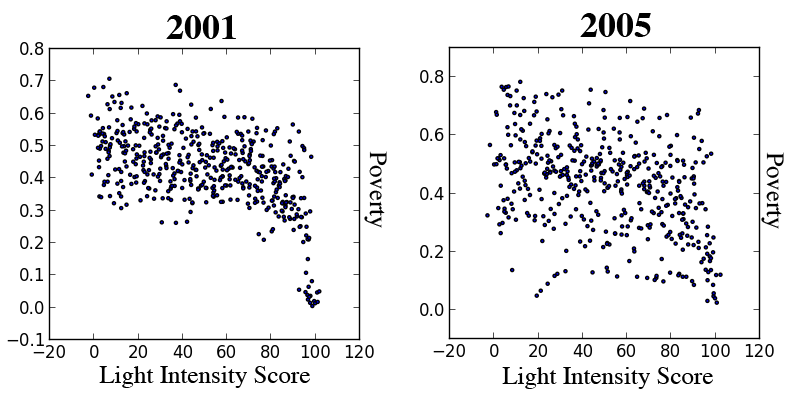
\includegraphics[width=0.8\textwidth]{figures/light-vs-poverty}
  \caption{Light Intensity Score vs. Percentage of Population in Poverty for all Upazilas.  Notice that in 2001, an increase in light intensity corresponds closely to a decrease in average poverty, particularly for the brightest Upazilas. On the other hand,  this correlation is far less evident in 2005, after the devastating 2004 tsunami.}
  \label{fig:light-vs-poverty}
\end{figure}

\begin{figure}
  \centering
  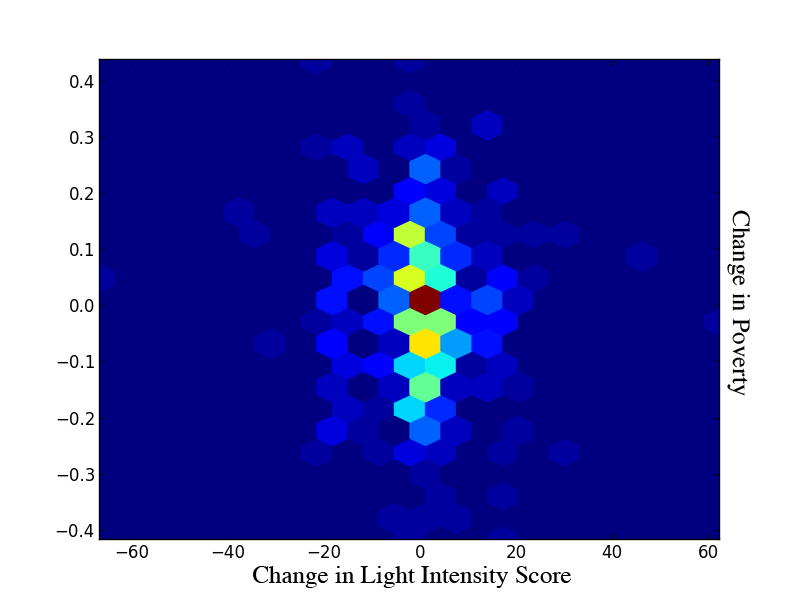
\includegraphics[width=0.5\textwidth]{figures/dlight-vs-dpoverty}
  \caption{Change in Light Intensity Score vs. Change Percentage of Population in Poverty between 2005 and 2001 as a 2 dimensional histogram over Upazilas. No correlation between the two is evident.}
  \label{fig:dlight-vs-dpoverty}
\end{figure}

  Our initial task was to determine if light intensity was at all indicative of poverty. As can be seen in Figure \ref{fig:light-vs-poverty}, there is indeed a correlation between these two variables, particularly near the brightest Upazilas. Indeed, the brightest Upazilas encompass the area surrounding the capital city of Dhaka are also the areas with the least amount of poverty.  In 2005, however, the correlation is far less clear.  The primary cause we believe is the tsunami of 2004, which markedly increased the amount of poverty in coastal regions.  
  
  On the other hand, Figure \ref{fig:dlight-vs-dpoverty} shows that change in light intensity and change in poverty (both between 2001 and 2005) appear entirely independent. Thus, we do not expect the former will allow us to predict the latter with any degree of accuracy.

%%%%%%%%%%%%%%%%%%%%%%%%%%%%%%%%%%%%%%%%%%%%%%%%%%%%%%%%%%%%%%%%%%%%%%%%%%
\subsection{Predicting Poverty}
%%%%%%%%%%%%%%%%%%%%%%%%%%%%%%%%%%%%%%%%%%%%%%%%%%%%%%%%%%%%%%%%%%%%%%%%%%

% | # | features | target | RMSE |
\begin{table}
  \centering
\begin{tabular}{| l | l | l | l |}
  \hline
  Figure                                          & Features                      & Prediction Target             & RMSE                      \\
  \hline
  N/A                                             & Bias                          & 2001 Poverty                  & 0.113242                  \\
  \hline
  \multirow{2}{*}{\ref{fig:poverty-predictions} Top Left}         & Bias                          & \multirow{2}{*}{2001 Poverty} & \multirow{2}{*}{0.087014} \\
                                                  & 2001 Light Intensity Score    &                               &                           \\
  \hline
  \multirow{3}{*}{\ref{fig:poverty-predictions} Top Right}  & Bias                          & \multirow{3}{*}{2001 Poverty} & \multirow{3}{*}{0.069896} \\
                                                  & 2001 Light Intensity Score    &                               &                           \\
                                                  & 2001 Census Features          &                               &                           \\
  \hline
  N/A                                             & Bias                          & 2005 Poverty                  & 0.166489                  \\
  \hline
  \multirow{2}{*}{\ref{fig:poverty-predictions} Bottom Left}         & Bias                          & \multirow{2}{*}{2005 Poverty} & \multirow{2}{*}{0.152265} \\
                                                  & 2005 Light Intensity Score    &                               &                           \\
  \hline
  \multirow{3}{*}{\ref{fig:poverty-predictions} Bottom Right}  & Bias                          & \multirow{3}{*}{2005 Poverty} & \multirow{3}{*}{0.129245} \\
                                                  & 2005 Light Intensity Score    &                               &                           \\
                                                  & 2001 Census Features          &                               &                           \\
  \hline
  N/A                                             & Bias                          & 2005 Poverty - 2001 Poverty   & 0.149903                  \\
  \hline
  \multirow{4}{*}{\ref{fig:dpoverty-predictions} Left}        & Bias                          & \multirow{4}{*}{2005 Poverty - 2001 Poverty} & \multirow{4}{*}{0.145950} \\
                                                  & 2001 Light Intensity Score    &                               &                           \\
                                                  & 2001 Poverty                  &                               &                           \\
                                                  & 2005 Light Intensity Score    &                               &                           \\
  \hline
  \multirow{5}{*}{\ref{fig:dpoverty-predictions} Right}  & Bias                          & \multirow{5}{*}{2005 Poverty - 2001 Poverty} & \multirow{5}{*}{0.129603} \\
                                                  & 2001 Light Intensity Score    &                               &                           \\
                                                  & 2001 Census Features          &                               &                           \\
                                                  & 2001 Poverty                  &                               &                           \\
                                                  & 2005 Light Intensity Score    &                               &                           \\
  \hline
\end{tabular}
\caption{Root Mean Squared Error on held out data for all experiments.}
\label{tbl:results}
\end{table}

\begin{figure}
  \centering
  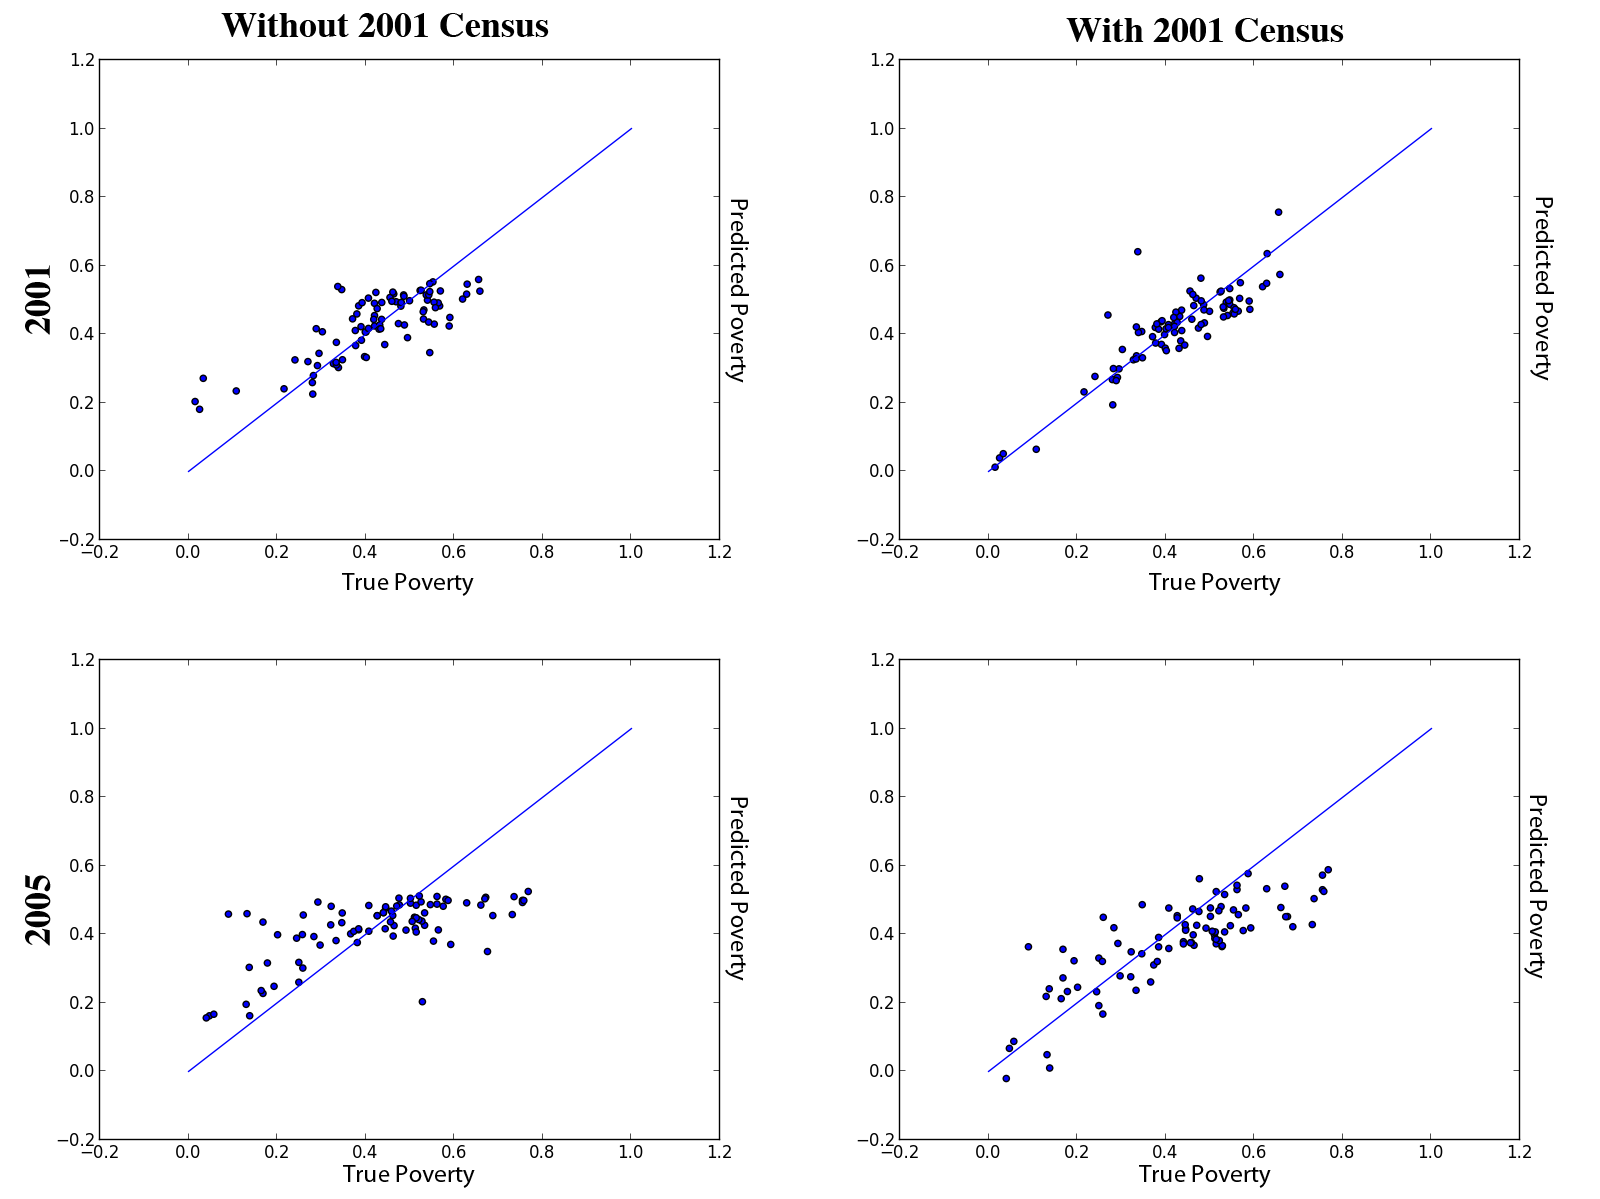
\includegraphics[width=0.95\textwidth]{figures/poverty-predictions}
  \caption{Predicted and True Poverty levels on held out data. The top row predicts the percentage of population in poverty in each Upazila in 2001 and the bottom row in 2005. The left column only uses Bias and Light Intesity Score features and the right also includes 2001 census features.}
  \label{fig:poverty-predictions}
\end{figure}

  Our second task was to build a predictive model for poverty.  The model chose for this task is Linear Regression augmented with a quadratic regularization term, most commonly known as Ridge Regression. In these experiments, our input is a set of features for each Upazila, and our desired output is the percentage of population in poverty. We set aside 20\% of the Upazilas to validate our model, and use 5-way cross validation on the remaining 80\% to select model parameters.  All features are normalized by subtracting their mean and dividing by their standard deviations, as is typical in Linear Regression.  In addition, a constant bias term is added to account for the average poverty across all Upazilas.
  
  We are happy to report that our initial model using Bias and Light Intensity Score features is already surprisingly accurate for 2001 (See Figure \ref{fig:poverty-predictions} and Table \ref{tbl:results}). When using only a bias feature (that is, no information at all), we obtain a Root Mean Squared Error of 0.113, but with the addition of Light Intensity, that error drops to 0.087. When 2001 census features are also included, that error further decreases to 0.0700.  In 2005, where light intensity was observed to be less correlated with poverty, we see only a slight drop in error compared to the bias-only baseline (0.152 vs. 0.166).  With the addition of 2001 census features, that error again reduces to 0.129.  
  
%%%%%%%%%%%%%%%%%%%%%%%%%%%%%%%%%%%%%%%%%%%%%%%%%%%%%%%%%%%%%%%%%%%%%%%%%%
\subsection{Predicting Change in Poverty}
%%%%%%%%%%%%%%%%%%%%%%%%%%%%%%%%%%%%%%%%%%%%%%%%%%%%%%%%%%%%%%%%%%%%%%%%%%

\begin{figure}
  \centering
  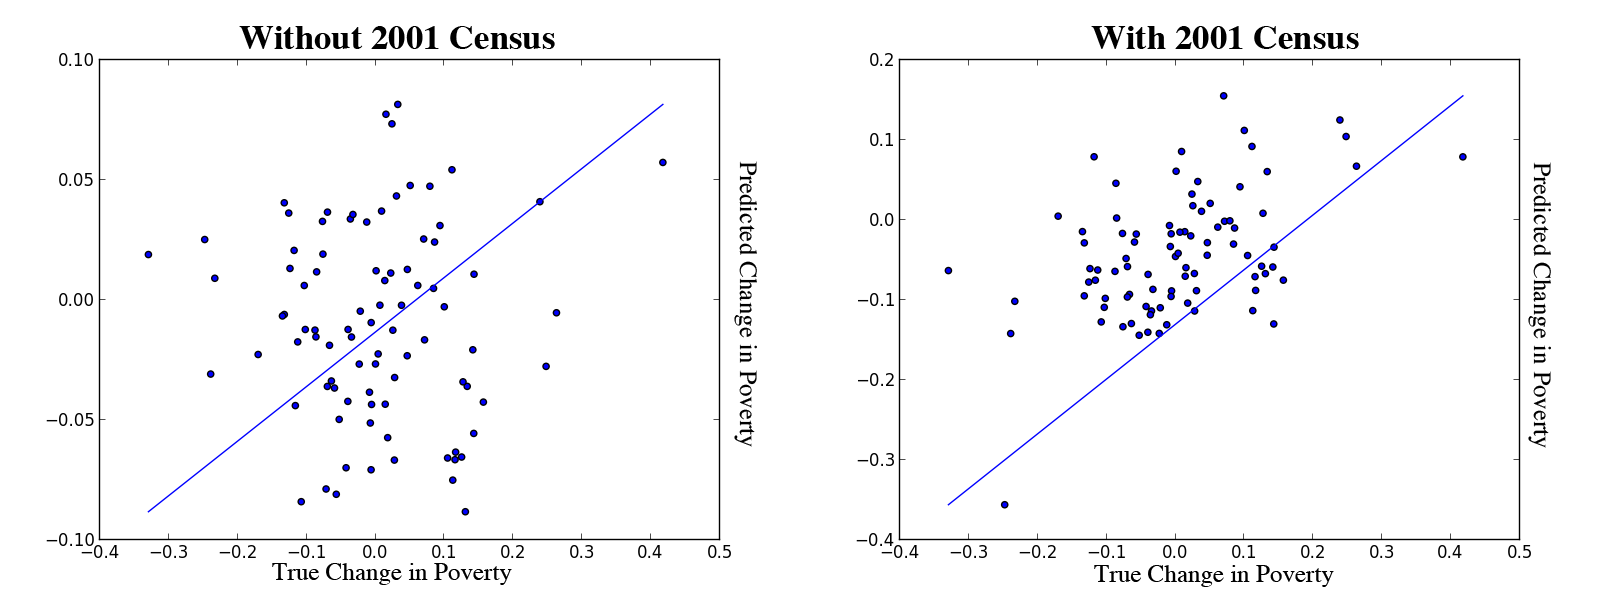
\includegraphics[width=0.95\textwidth]{figures/dpoverty-predictions}
  \caption{Predicted and True Poverty Change.  The left figure uses bias, 2001 and 2005 light intensity scores, and 2001 poverty levels as features, whereas the right also uses 2001 census features.}
  \label{fig:dpoverty-predictions}
\end{figure}

  Our final task is to predict \textit{change} in poverty using change in light intensity. Our initial analysis showed that the two were uncorrelated, and our attempts at predicting the latter using the former were unsuccessful.  Using light intensity features, we obtain minimal decrease in accuracy over the baseline (0.146 vs. 0.150). When 2001 census features are also added, that error drops to 0.130.  Figure \ref{fig:dpoverty-predictions} reveals that the decrease in error is not significant enough to merit use.

%%%%%%%%%%%%%%%%%%%%%%%%%%%%%%%%%%%%%%%%%%%%%%%%%%%%%%%%%%%%%%%%%%%%%%%%%%	
\section{Related Work}
%%%%%%%%%%%%%%%%%%%%%%%%%%%%%%%%%%%%%%%%%%%%%%%%%%%%%%%%%%%%%%%%%%%%%%%%%%

\todo{Who else has tried to predict poverty via alternative measures?}

\todo{How did they do?}

%%%%%%%%%%%%%%%%%%%%%%%%%%%%%%%%%%%%%%%%%%%%%%%%%%%%%%%%%%%%%%%%%%%%%%%%%%		
\section{Conclusion}
%%%%%%%%%%%%%%%%%%%%%%%%%%%%%%%%%%%%%%%%%%%%%%%%%%%%%%%%%%%%%%%%%%%%%%%%%%

\todo{What were our limitations?}

\todo{Is lighting a good indicator?}

  In this work, we explored the potential use of night time illumination photos in predicting poverty levels. We experiment using such photos and poverty census data collected in Bangladesh in 2001 and 2005, and find that Ridge Regression is very capable of predicting the latter using the former before the 2004 tsunami but is less capable after. We further find that change in light intensity is uncorrelated with change in poverty and is thus insufficient information for prediction.
  
  Looking forward, we recommend that three avenues be taken. The first is the addition of other cheaply obtainable indicators of poverty. We stress that such indicators need not be exactly representative of poverty, only that they be correlated. If such features are correlated with aspects of poverty or wealth, their addition can only strengthen our predictions.  Secondly, we recommend further evaluation on other models aside from Ridge Regression (which was chosen primarily for its availability).  Indeed, Linear Regression may predict values outside of 0 and 1, making it ill-suited for the given task.  Finally, we recommend additional experiments be done on datasets larger than 2 years of Bangladesh alone.  Poverty census data is doubtless available for other countries, and NOAA satellite imagery encompasses the entire planet. 

%%%%%%%%%%%%%%%%%%%%%%%%%%%%%%%%%%%%%%%%%%%%%%%%%%%%%%%%%%%%%%%%%%%%%%%%%%	
\end{document}
